\documentclass[fleqn]{article}
\usepackage[utf8]{inputenc}
\usepackage{proof}
\usepackage{amsmath,stmaryrd}
\usepackage{eufrak}
\usepackage[a4paper,showframe]{geometry}
\usepackage{graphicx}
\usepackage[final]{pdfpages}

\newtheorem{theorem}{Theorem}

\begin{document}

\section{Source}

\[
\scriptsize
\begin{array}{rcl}
    c,\tau,i & ::= & \alpha \mid CC \mid o_{ui}~i \mid i~o_{bi}~i \mid i~?~i:i \mid \mathbf{TimeAbs}~\alpha. i \mid \mathbf{TimeApp}_n~c~i \\
    & \mid & \tau \times \tau \mid \tau + \tau \mid \tau \xrightarrow{i} \tau \mid \lambda \alpha :: \kappa. \tau \mid \tau~c \mid \forall \alpha :: \kappa. \tau \mid \exists \alpha :: \kappa. \tau \mid \mu \alpha :: \kappa. \tau \\
    & \mid & \mathbf{1} \mid \mathbf{nat}~i \mid \mathbf{arr}~\tau~i \\
    s & ::= & \mathbf{Nat} \mid \mathbf{1} \mid \mathbf{2} \mid \mathbf{TimeFun}_n \\
    \kappa & ::= & \star \mid \kappa \Rightarrow \kappa \mid s \mid \{ \alpha :: \kappa \mid p \} \\
    p & ::= & \top \mid \bot \mid p~o_{bc}~p \mid \neg p \mid i~o_{br}~i \mid \forall \alpha :: s. p \mid \exists \alpha :: s. p \\
    e & ::= & x \mid EC \mid \lambda x:\tau. e \mid e~e \mid (e,e) \mid e.\mathbf{1} \mid e.\mathbf{2} \mid \mathbf{l}.e \mid \mathbf{r}.e \mid \mathbf{case}~e~x.e~x.e \mid \mathbf{fold}~e \mid \mathbf{unfold}~e \\
    & \mid & \mathbf{pack}\langle c \mid e \rangle \mid \mathbf{unpack}~e~\alpha.x.e \mid \Lambda \alpha :: \kappa. e \mid e~c \mid e~o_{bt}~e \mid \mathbf{rec}_\tau~x.e \mid \mathbf{let}~x=e~\mathbf{in}~e \\
    & \mid & \mathbf{new}~e~e \mid e[e] \mid e[e] := e
\end{array}
\]

\[
\scriptsize
\begin{array}{l}
    \mathcal{K} \vdash \kappa_1 \equiv \kappa_2 \\
    \infer[\textsc{KdEqType}]{\mathcal{K} \vdash \star \equiv \star}{} \hspace{1em}
    \infer[\textsc{KdEqArrow}]{\mathcal{K} \vdash \kappa_{11} \Rightarrow \kappa_{12} \equiv \kappa_{21} \Rightarrow \kappa_{22}}{\mathcal{K} \vdash \kappa_{11} \equiv \kappa_{21} & \mathcal{K} \vdash \kappa_{12} \equiv \kappa_{22}} \\
    \infer[\textsc{KdEqBaseSort}]{\mathcal{K} \vdash s \equiv s}{} \hspace{1em}
    \infer[\textsc{KdEqSubset}]{\mathcal{K} \vdash \{ \alpha :: \kappa_{11} \mid p_{12} \} \equiv \{ \alpha :: \kappa_{21} \mid p_{22} \}}{\mathcal{K} \vdash \kappa_{11} \equiv \kappa_{21} & \mathcal{K}, \alpha :: \kappa_{11} \vdash p_{12} \Leftrightarrow p_{22}} \\
    \infer[\textsc{KdEqSubsetElimLeft}]{\mathcal{K} \vdash \{ \alpha :: \kappa \mid p \} \equiv \kappa}{\mathcal{K},\alpha :: \kappa \vdash p} \hspace{1em}
    \infer[\textsc{KdEqSubsetElimRight}]{\mathcal{K} \vdash \kappa \equiv \{ \alpha :: \kappa \mid p \}}{\mathcal{K},\alpha :: \kappa \vdash p}
\end{array}
\]

\[
\scriptsize
\begin{array}{l}
    \mathcal{K} \vdash \mathrm{wf}~\kappa \\
    \infer[\textsc{WfKdType}]{\mathcal{K} \vdash \mathrm{wf}~\star}{} \hspace{1em}
    \infer[\textsc{WfKdArrow}]{\mathcal{K} \vdash \mathrm{wf}~\kappa_1 \Rightarrow \kappa_2}{\mathcal{K} \vdash \mathrm{wf}~\kappa_1 & \mathcal{K} \vdash \mathrm{wf}~\kappa_2} \\
    \infer[\textsc{WfKdBaseSort}]{\mathcal{K} \vdash \mathrm{wf}~s}{} \hspace{1em}
    \infer[\textsc{WfKdSubset}]{\mathcal{K} \vdash \mathrm{wf}~\{ \alpha :: \kappa \mid p \}}{\mathcal{K},\alpha :: \kappa \vdash \mathrm{wf}~p}
\end{array}
\]

\[
\scriptsize
\begin{array}{l}
    \mathcal{K} \vdash \mathrm{wf}~p \\
    \infer[\textsc{WfPropTrue}]{\mathcal{K} \vdash \mathrm{wf}~\top}{} \hspace{1em}
    \infer[\textsc{WfPropFalse}]{\mathcal{K} \vdash \mathrm{wf}~\bot}{} \\
    \infer[\textsc{WfPropBinConn}]{\mathcal{K} \vdash \mathrm{wf}~p_1~o_{bc}~p_2}{\mathcal{K} \vdash \mathrm{wf}~p_1 & \mathcal{K} \vdash \mathrm{wf}~p_2} \hspace{1em}
    \infer[\textsc{WfPropNot}]{\mathcal{K} \vdash \mathrm{wf}~\neg p}{\mathcal{K} \vdash \mathrm{wf}~p} \hspace{1em} \hspace{1em}
    \infer[\textsc{WfPropBinRel}]{\mathcal{K} \vdash \mathrm{wf}~i_1~o_{br}~i_2}{\mathcal{K} \vdash i_1 :: o_{br}.\kappa_1 & \mathcal{K} \vdash i_2 :: o_{br}.\kappa_2} \\
    \infer[\textsc{WfPropForall}]{\mathcal{K} \vdash \mathrm{wf}~\forall \alpha :: s. p}{\mathcal{K},\alpha :: s \vdash \mathrm{wf}~p} \hspace{1em}
    \infer[\textsc{WfPropExists}]{\mathcal{K} \vdash \mathrm{wf}~\exists \alpha :: s. p}{\mathcal{K},\alpha :: s \vdash \mathrm{wf}~p}
\end{array}
\]

\[
\scriptsize
\begin{array}{l}
    \mathcal{K} \vdash c :: \kappa \\
    \infer[\textsc{KdVar}]{\mathcal{K} \vdash \alpha :: \kappa}{\mathcal{K}(\alpha)=\kappa} \hspace{1em}
    \infer[\textsc{KdConst}]{\mathcal{K} \vdash CC :: kind(CC)}{} \hspace{1em}
    \infer[\textsc{KdUnOp}]{\mathcal{K} \vdash o_{ui}~i :: o_{ui}.\kappa_r}{\mathcal{K} \vdash i :: o_{ui}.\kappa_a} \\
    \infer[\textsc{KdBinOp}]{\mathcal{K} \vdash i_1~o_{bi}~i_2 :: o_{bi}.\kappa_r}{\mathcal{K} \vdash i_1 :: o_{bi}.\kappa_1 & \mathcal{K} \vdash i_2 :: o_{bi}.\kappa_2} \hspace{1em}
    \infer[\textsc{KdIte}]{\mathcal{K} \vdash i~?~i_1 : i_2 :: \kappa}{\mathcal{K} \vdash i :: \mathbf{2} & \mathcal{K} \vdash i_1 :: \kappa & \mathcal{K} \vdash i_2 :: \kappa} \\
    \infer[\textsc{KdTimeAbs}]{\mathcal{K} \vdash \mathbf{TimeAbs}~\alpha. i :: \mathbf{TimeFun}_{n + 1}}{\mathcal{K},\alpha :: \mathbf{Nat} \vdash i :: \mathbf{TimeFun}_n & \mathbf{TimeAbs}~\alpha. i~\mathrm{is}~\mathrm{monotone}} \\
    \infer[\textsc{KdTimeApp}]{\mathcal{K} \vdash \mathbf{TimeApp}_n~c~i :: \mathbf{TimeFun}_n}{\mathcal{K} \vdash c :: \mathbf{TimeFun}_{n+1} & \mathcal{K} \vdash i :: \mathbf{Nat}} \hspace{1em}
    \infer[\textsc{KdProd}]{\mathcal{K} \vdash \tau_1 \times \tau_2 :: \star}{\mathcal{K} \vdash \tau_1 :: \star & \mathcal{K} \vdash \tau_2 :: \star} \\
    \infer[\textsc{KdSum}]{\mathcal{K} \vdash \tau_1 + \tau_2 :: \star}{\mathcal{K} \vdash \tau_1 :: \star & \mathcal{K} \vdash \tau_2 :: \star} \hspace{1em}
    \infer[\textsc{KdArrow}]{\mathcal{K} \vdash \tau_1 \xrightarrow{i} \tau_2 :: \star}{\mathcal{K} \vdash \tau_1 :: \star & \mathcal{K} \vdash \tau_2 :: \star & \mathcal{K} \vdash i :: \mathbf{TimeFun}_0} \\
    \infer[\textsc{KdAbs}]{\mathcal{K} \vdash \lambda \alpha :: \kappa. \tau :: \kappa \Rightarrow \kappa_1}{\mathcal{K} \vdash \mathrm{wf}~\kappa & \mathcal{K},\alpha :: \kappa \vdash \tau :: \kappa_1} \hspace{1em}
    \infer[\textsc{KdApp}]{\mathcal{K} \vdash \tau~c :: \kappa_2}{\mathcal{K} \vdash \tau :: \kappa_1 \Rightarrow \kappa_2 & \mathcal{K} \vdash c :: \kappa_1} \\
    \infer[\textsc{KdForall}]{\mathcal{K} \vdash \forall \alpha :: \kappa. \tau :: \star}{\mathcal{K} \vdash \mathrm{wf}~\kappa & \mathcal{K},\alpha :: \kappa \vdash \tau :: \star} \hspace{1em}
    \infer[\textsc{KdExists}]{\mathcal{K} \vdash \exists \alpha :: \kappa. \tau :: \star}{\mathcal{K} \vdash \mathrm{wf}~\kappa & \mathcal{K},\alpha :: \kappa \vdash \tau :: \star} \\
    \infer[\textsc{KdRec}]{\mathcal{K} \vdash \mu \alpha :: \kappa. \tau :: \kappa}{\mathcal{K} \vdash \mathrm{wf}~\kappa & \mathcal{K},\alpha :: \kappa \vdash \tau :: \kappa} \hspace{1em}
    \infer[\textsc{KdTypeUnit}]{\mathcal{K} \vdash \mathbf{1} :: \star}{} \hspace{1em}
    \infer[\textsc{KdTypeNat}]{\mathcal{K} \vdash \mathbf{nat}~i :: \star}{\mathcal{K} \vdash i :: \mathbf{Nat}} \\
    \infer[\textsc{KdTypeArr}]{\mathcal{K} \vdash \mathbf{arr}~\tau~i :: \star}{\mathcal{K} \vdash \tau :: \star & \mathcal{K} \vdash i :: \mathbf{Nat}} \hspace{1em}
    \infer[\textsc{KdEq}]{\mathcal{K} \vdash c :: \kappa_2}{\mathcal{K} \vdash c :: \kappa_1 & \mathcal{K} \vdash \kappa_1 \equiv \kappa_2}
\end{array}
\]

\[
\scriptsize
\begin{array}{l}
    \mathcal{K} \vdash c_1 \equiv c_2 \\
    \infer[\textsc{TyEqVar}]{\mathcal{K} \vdash \alpha \equiv \alpha}{} \hspace{1em}
    \infer[\textsc{TyEqConst}]{\mathcal{K} \vdash CC \equiv CC}{} \hspace{1em}
    \infer[\textsc{TyEqUnOp}]{\mathcal{K} \vdash o_{ui}~i_1 \equiv o_{ui}~i_2}{\mathcal{K} \vdash i_1 \equiv i_2} \\
    \infer[\textsc{TyEqBinOp}]{\mathcal{K} \vdash i_{11}~o_{bi}~i_{12} \equiv i_{21}~o_{bi}~i_{22}}{\mathcal{K} \vdash i_{11} \equiv i_{21} & \mathcal{K} \vdash i_{12} \equiv i_{22}} \hspace{1em}
    \infer[\textsc{TyEqIte}]{\mathcal{K} \vdash i_{11}~?~i_{12} : i_{13} \equiv i_{21}~?~i_{22} : i_{23}}{\mathcal{K} \vdash i_{11} \equiv i_{21} & \mathcal{K} \vdash i_{12} \equiv i_{22} & \mathcal{K} \vdash i_{13} \equiv i_{23}} \\
    \infer[\textsc{TyEqTimeAbs}]{\mathcal{K} \vdash \mathbf{TimeAbs}~\alpha. i \equiv \mathbf{TimeAbs}~\alpha. i}{} \hspace{1em}
    \infer[\textsc{TyEqTimeApp}]{\mathcal{K} \vdash \mathbf{TimeApp}_n~c~i \equiv \mathbf{TimeApp}_n~c~i}{} \\
    \infer[\textsc{TyEqProd}]{\mathcal{K} \vdash \tau_{11} \times \tau_{12} \equiv \tau_{21} \times \tau_{22}}{\mathcal{K} \vdash \tau_{11} \equiv \tau_{21} & \mathcal{K} \vdash \tau_{12} \equiv \tau_{22}} \hspace{1em}
    \infer[\textsc{TyEqSum}]{\mathcal{K} \vdash \tau_{11} + \tau_{12} \equiv \tau_{21} + \tau_{22}}{\mathcal{K} \vdash \tau_{11} \equiv \tau_{21} & \mathcal{K} \vdash \tau_{12} \equiv \tau_{22}} \\
    \infer[\textsc{TyEqArrow}]{\mathcal{K} \vdash \tau_{11} \xrightarrow{i_1} \tau_{12} \equiv \tau_{21} \xrightarrow{i_2} \tau_{22}}{\mathcal{K} \vdash \tau_{11} \equiv \tau_{21} & \mathcal{K} \vdash i_1 =_r i_2 & \mathcal{K} \vdash \tau_{12} \equiv \tau_{22}} \\
    \infer[\textsc{TyEqAbs}]{\mathcal{K} \vdash \lambda \alpha :: \kappa. \tau \equiv \lambda \alpha :: \kappa. \tau}{} \hspace{1em}
    \infer[\textsc{TyEqApp}]{\mathcal{K} \vdash \tau_{1}~c_{1} \equiv \tau_{2}~c_{2}}{\mathcal{K} \vdash \tau_{1} \equiv \tau_{2} & \mathcal{K} \vdash c_{1} \equiv c_{2}} \\
    \infer[\textsc{TyEqBeta}]{\mathcal{K} \vdash (\lambda \alpha :: \kappa. \tau_1)~\tau_2 \equiv \tau_1[\tau_2/\alpha]}{} \hspace{1em}
    \infer[\textsc{TyEqBetaRev}]{\mathcal{K} \vdash \tau_1[\tau_2/\alpha] \equiv (\lambda \alpha :: \kappa. \tau_1)~\tau_2}{} \\
    \infer[\textsc{TyEqForall}]{\mathcal{K} \vdash \forall \alpha :: \kappa_1. \tau_1 \equiv \forall \alpha :: \kappa_2. \tau_2}{\mathcal{K} \vdash \kappa_1 \equiv \kappa_2 & \mathcal{K},\alpha :: \kappa_1 \vdash \tau_1 \equiv \tau_2} \hspace{1em}
    \infer[\textsc{TyEqExists}]{\mathcal{K} \vdash \exists \alpha :: \kappa_1. \tau_1 \equiv \exists \alpha :: \kappa_2. \tau_2}{\mathcal{K} \vdash \kappa_1 \equiv \kappa_2 & \mathcal{K},\alpha :: \kappa_1 \vdash \tau_1 \equiv \tau_2} \\
    \infer[\textsc{TyEqRec}]{\mathcal{K} \vdash \mu \alpha :: \kappa_1. \tau_1 \equiv \mu \alpha :: \kappa_2. \tau_2}{\mathcal{K} \vdash \kappa_1 \equiv \kappa_2 & \mathcal{K},\alpha :: \kappa_1 \vdash \tau_1 \equiv \tau_2} \hspace{1em}
    \infer[\textsc{TyEqTypeUnit}]{\mathcal{K} \vdash \mathbf{1} \equiv \mathbf{1}}{} \hspace{1em}
    \infer[\textsc{TyEqTypeNat}]{\mathcal{K} \vdash \mathbf{nat}~i_1 \equiv \mathbf{nat}~i_2}{\mathcal{K} \vdash i_1 =_n i_2} \\
    \infer[\textsc{TyEqTypeArr}]{\mathcal{K} \vdash \mathbf{arr}~\tau_1~i_1 \equiv \mathbf{arr}~\tau_2~i_2}{\mathcal{K} \vdash \tau_1 \equiv \tau_2 & \mathcal{K} \vdash i_1 =_n i_2} \hspace{1em}
    \infer[\textsc{TyEqTrans}]{\mathcal{K} \vdash c_1 \equiv c_3}{\mathcal{K} \vdash c_1 \equiv c_2 & \mathcal{K} \vdash c_2 \equiv c_3} \\
    \infer[\textsc{TyEqNat}]{\mathcal{K} \vdash i_1 \equiv i_2}{\mathcal{K} \vdash i_1 =_n i_2} \hspace{1em}
    \infer[\textsc{TyEqTime}]{\mathcal{K} \vdash i_1 \equiv i_2}{\mathcal{K} \vdash i_1 =_r i_2}
\end{array}
\]

\[
\scriptsize
\begin{array}{l}
    \vdash \mathrm{value}~e \\
    \infer[\textsc{VConst}]{\vdash \mathrm{value}~EC}{} \hspace{1em}
    \infer[\textsc{VPair}]{\vdash \mathrm{value}~(e_1,e_2)}{\vdash \mathrm{value}~e_1 & \vdash \mathrm{value}~e_2} \hspace{1em}
    \infer[\textsc{VInl}]{\vdash \mathrm{value}~\mathbf{l}.e}{\vdash \mathrm{value}~e} \hspace{1em}
    \infer[\textsc{VInr}]{\vdash \mathrm{value}~\mathbf{r}.e}{\vdash \mathrm{value}~e} \\
    \infer[\textsc{VAbs}]{\vdash \mathrm{value}~\lambda x : \tau.e}{} \hspace{1em}
    \infer[\textsc{VAbsC}]{\vdash \mathrm{value}~\Lambda \alpha :: \kappa.e}{} \hspace{1em}
    \infer[\textsc{VPack}]{\vdash \mathrm{value}~\mathbf{pack}\langle c \mid e \rangle}{\vdash \mathrm{value}~e} \hspace{1em}
    \infer[\textsc{VFold}]{\vdash \mathrm{value}~\mathbf{fold}~e}{\vdash \mathrm{value}~e}
\end{array}
\]

\[
\scriptsize
\begin{array}{l}
    (\mathcal{K}; \mathcal{T}) \vdash e : \tau \triangleright i \\
    \infer[\textsc{TyVar}]{\mathcal{C} \vdash x : \tau \triangleright 0}{\mathcal{C}.2(x)=\tau} \hspace{1em}
    \infer[\textsc{TyConst}]{\mathcal{C} \vdash EC : type(EC) \triangleright 0}{} \\
    \infer[\textsc{TyAbs}]{\mathcal{C} \vdash \lambda x:\tau. e : \tau \xrightarrow{i} \tau_1 \triangleright 0}{\mathcal{C}.1 \vdash \tau :: \star & \mathcal{C},x:\tau \vdash e : \tau_1 \triangleright i} \hspace{1em}
    \infer[\textsc{TyApp}]{\mathcal{C} \vdash e_1~e_2 : \tau_2 \triangleright i_1 + i_2 + 1 + i}{\mathcal{C} \vdash e_1 : \tau_1 \xrightarrow{i} \tau_2 \triangleright i_1 & \mathcal{C} \vdash e_2 : \tau_1 \triangleright i_2} \\
    \infer[\textsc{TyPair}]{\mathcal{C} \vdash (e_1,e_2) : \tau_1 \times \tau_2 \triangleright i_1 + i_2}{\mathcal{C} \vdash e_1 : \tau_1 \triangleright i_1 & \mathcal{C} \vdash e_2 : \tau_2 \triangleright i_2} \hspace{1em}
    \infer[\textsc{TyFst}]{\mathcal{C} \vdash e.\mathbf{1} : \tau_1 \triangleright i}{\mathcal{C} \vdash e : \tau_1 \times \tau_2 \triangleright i} \hspace{1em}
    \infer[\textsc{TySnd}]{\mathcal{C} \vdash e.\mathbf{2} : \tau_2 \triangleright i}{\mathcal{C} \vdash e : \tau_1 \times \tau_2 \triangleright i} \\
    \infer[\textsc{TyInl}]{\mathcal{C} \vdash \mathbf{l}.e : \tau_1 + \tau_2 \triangleright i}{\mathcal{C} \vdash e : \tau_1 \triangleright i & \mathcal{C}.1 \vdash \tau_2 :: \star} \hspace{1em}
    \infer[\textsc{TyInr}]{\mathcal{C} \vdash \mathbf{r}.e : \tau_1 + \tau_2 \triangleright i}{\mathcal{C} \vdash e : \tau_2 \triangleright i & \mathcal{C}.1 \vdash \tau_1 :: \star} \\
    \infer[\textsc{TyCase}]{\mathcal{C} \vdash \mathbf{case}~e~x.e_1~x.e_2 : \tau \triangleright i + \max(i_1,i_2)}{\mathcal{C} \vdash e : \tau_1 + \tau_2 \triangleright i & \mathcal{C},x:\tau_m \vdash e_m : \tau \triangleright i_m} \\
    \infer[\textsc{TyFold}]{\mathcal{C} \vdash \mathbf{fold}~e : \tau~\vec{c} \triangleright i}{\mathcal{C}.1 \vdash \tau~\vec{c} :: \star & \tau = \mu \alpha :: \kappa. \tau_1 & \mathcal{C} \vdash e : \tau_1[\tau/\alpha]~\vec{c} \triangleright i} \hspace{1em}
    \infer[\textsc{TyUnfold}]{\mathcal{C} \vdash \mathbf{unfold}~e : \tau_1[\tau/\alpha]~\vec{c} \triangleright i}{\tau = \mu \alpha :: \kappa. \tau_1 & \mathcal{C} \vdash e : \tau~\vec{c} \triangleright i} \\
    \infer[\textsc{TyPack}]{\mathcal{C} \vdash \mathbf{pack}\langle c \mid e \rangle : \exists \alpha :: \kappa. \tau \triangleright i}{\mathcal{C}.1 \vdash \exists \alpha :: \kappa. \tau :: \star & \mathcal{C}.1 \vdash c :: \kappa & \mathcal{C} \vdash e : \tau[c/\alpha] \triangleright i} \\
    \infer[\textsc{TyUnpack}]{\mathcal{C} \vdash \mathbf{unpack}~e_1~\alpha.x.e_2 : \tau_2 \triangleright i_1 + i_2}{\mathcal{C} \vdash e_1 : \exists \alpha :: \kappa. \tau \triangleright i_1 & \mathcal{C},\alpha::\kappa,x:\tau \vdash e_2 : \tau_2 \triangleright i_2 & \tau_2,i_2~\mathrm{do~not~contain}~\alpha} \\
    \infer[\textsc{TyAbsC}]{\mathcal{C} \vdash \Lambda \alpha :: \kappa. e : \forall \alpha :: \kappa. \tau \triangleright 0}{\mathcal{C}.1 \vdash \mathrm{wf}~\kappa & \vdash \mathrm{value}~e & \mathcal{C},\alpha :: \kappa \vdash e : \tau \triangleright 0} \hspace{1em}
    \infer[\textsc{TyAppC}]{\mathcal{C} \vdash e~c : \tau[c/\alpha] \triangleright i}{\mathcal{C} \vdash e : \forall \alpha :: \kappa. \tau \triangleright i & \mathcal{C}.1 \vdash c :: \kappa} \\
    \infer[\textsc{TyBinOp}]{\mathcal{C} \vdash e_1~o_{bt}~e_2 : o_{bt}.\tau_r \triangleright i_1 + i_2}{\mathcal{C} \vdash e_1 : o_{bt}.\tau_1 \triangleright i_1 & \mathcal{C} \vdash e_2 : o_{bt}.\tau_2 \triangleright i_2} \hspace{1em}
    \infer[\textsc{TyRec}]{\mathcal{C} \vdash \mathbf{rec}_\tau~x. e : \tau \triangleright 0}{e = \Lambda \overrightarrow{\alpha :: \kappa}. \lambda y : \tau_y. e_1 & \mathcal{C}.1 \vdash \tau :: \star & \mathcal{C},x:\tau \vdash e : \tau \triangleright 0} \\
    \infer[\textsc{TyLet}]{\mathcal{C} \vdash \mathbf{let}~x=e_1~\mathbf{in}~e_2 : \tau_2 \triangleright i_1 + i_2}{\mathcal{C} \vdash e_1 : \tau_1 \triangleright i_1 & \mathcal{C},x:\tau_1 \vdash e_2 : \tau_2 \triangleright i_2} \hspace{1em}
    \infer[\textsc{TyNew}]{\mathcal{C} \vdash \mathbf{new}~e_1~e_2 : \mathbf{arr}~\tau~j \triangleright i_1 + i_2}{\mathcal{C} \vdash e_1 : \tau \triangleright i_1 & \mathcal{C} \vdash e_2 : \mathbf{nat}~j \triangleright i_2} \\
    \infer[\textsc{TyRead}]{\mathcal{C} \vdash e_1[e_2] : \tau \triangleright i_1 + i_2}{\mathcal{C} \vdash e_1 : \mathbf{arr}~\tau~j_1 \triangleright i_1 & \mathcal{C} \vdash e_2 : \mathbf{nat}~j_2 \triangleright i_2 & \mathcal{C}.1 \vdash j_2 <_n j_1} \\
    \infer[\textsc{TyWrite}]{\mathcal{C} \vdash e_1[e_2] := e_3 : \mathbf{1} \triangleright i_1 + i_2 + i_3}{\mathcal{C} \vdash e_1 : \mathbf{arr}~\tau~j_1 \triangleright i_1 & \mathcal{C} \vdash e_2 : \mathbf{nat}~j_2 \triangleright i_2 & \mathcal{C}.1 \vdash j_2 <_n j_1 & \mathcal{C} \vdash e_3 : \tau \triangleright i_3} \\
    \infer[\textsc{TySub}]{\mathcal{C} \vdash e : \tau_2 \triangleright i_2}{\mathcal{C} \vdash e : \tau_1 \triangleright i_1 & \mathcal{C}.1 \vdash \tau_1 \equiv \tau_2 & \mathcal{C}.1 \vdash i_1 \le_r i_2}
\end{array}
\]
\section{CPS}

\newcommand{\cpsc}[1]{\mathfrak{K}_{\mathrm{cstr}}\llbracket #1 \rrbracket}
\newcommand{\cpst}[2]{\mathfrak{K}_{\mathrm{term}}\llbracket #1 \rrbracket ( #2 )}

\[
\scriptsize
\begin{array}{lcl}
    \cpsc{c} \\
    \cpsc{\alpha} & = & \alpha \\
    \cpsc{CC} & = & CC \\
    \cpsc{o_{ui}~i} & = & o_{ui}~\cpsc{i} \\
    \cpsc{i_1~o_{bi}~i_2} & = & \cpsc{i_1}~o_{bi}~\cpsc{i_2} \\
    \cpsc{i~?~i_1 : i_2} & = & \cpsc{i}~?~\cpsc{i_1} : \cpsc{i_2} \\
    \cpsc{\mathbf{TimeAbs}~\alpha.i} & = & \mathbf{TimeAbs}~\alpha.\cpsc{i} \\
    \cpsc{\mathbf{TimeApp}_n~c~i} & = & \mathbf{TimeApp}_n~\cpsc{c}~\cpsc{i} \\
    \cpsc{\tau_1 \times \tau_2} & = & \cpsc{\tau_1} \times \cpsc{\tau_2} \\
    \cpsc{\tau_1 + \tau_2} & = & \cpsc{\tau_1} + \cpsc{\tau_2} \\
    \cpsc{\tau_1 \xrightarrow{i} \tau_2} & = & \forall j :: \mathbf{TimeFun}_0. \cpsc{\tau_1} \times (\cpsc{\tau_2} \xrightarrow{j} \mathbf{1}) \xrightarrow{i'} \mathbf{1} \\
    & & \mathrm{where}~i'= C(\cpsc{i}+1) + 2\cpsc{i} + 1 + j \\
    \cpsc{\lambda \alpha :: \kappa. \tau} & = & \lambda \alpha :: \kappa. \cpsc{\tau} \\
    \cpsc{\tau~c} = \cpsc{\tau}~\cpsc{c} \\
    \cpsc{\forall \alpha :: \kappa. \tau} & = & \forall \alpha :: \kappa. \forall j :: \mathbf{TimeFun}_0. (\cpsc{\tau} \xrightarrow{j} \mathbf{1}) \xrightarrow{1 + j} \mathbf{void} \\
    \cpsc{\exists \alpha :: \kappa. \tau} & = & \exists \alpha :: \kappa. \cpsc{\tau} \\
    \cpsc{\mu \alpha :: \kappa. \tau} & = & \mu \alpha :: \kappa. \cpsc{\tau} \\
    \cpsc{\mathbf{1}} & = & \mathbf{1} \\
    \cpsc{\mathbf{nat}~i} & = & \mathbf{nat}~\cpsc{i} \\
    \cpsc{\mathbf{arr}~\tau~i} & = & \mathbf{arr}~\cpsc{\tau}~\cpsc{i}
\end{array}
\]

\newcommand{\jty}[4]{#1 \vdash #2 : #3 \triangleright #4}
\newcommand{\jtyc}[3]{#1 \vdash #2 : #3}

\[
\scriptsize
\begin{array}{lcl}
	\cpst{\jty{\mathcal{C}}{e}{\tau}{i}}{k} \\
	\cpst{\jty{\mathcal{C}}{x}{\tau}{0}}{k} & = & \mathrm{send}~k~x \\
	\cpst{\jty{\mathcal{C}}{EC}{\tau}{0}}{k} & = & \mathrm{send}~k~EC \\
	\cpst{\jty{\mathcal{C}}{\lambda x : \tau_1. e}{\tau_1 \xrightarrow{i} \tau_2}{0}}{k} & = & \mathrm{send}~k~(\Lambda j :: \mathbf{TimeFun}_0. \lambda y : \cpsc{\tau_1} \times (\cpsc{\tau_2} \xrightarrow{j} \mathbf{1}). \\
	& & ~~~~ (\mathbf{let}~c=y.\mathbf{2}~\mathbf{in} \\
	& & ~~~~~ \mathbf{let}~x=y.\mathbf{1}~\mathbf{in} \\
	& & ~~~~~ \cpst{\jty{\mathcal{C},x}{e}{\tau_2}{i}}{c}) \\
	& & ~~~~ \triangleright {C(\cpsc{i}+1)+2\cpsc{i}+1+j} ) \\
	\cpst{\jty{\mathcal{C}}{e_1~e_2}{\tau_2}{i_1+i_2+1+i}}{k} & = & \cpst{\jty{\mathcal{C}}{e_1}{\tau_1 \xrightarrow{i} \tau_2}{i_1}}{\lambda x_1 : \cpsc{\tau_1 \xrightarrow{i} \tau_2}. \\
	& & ~~~~ \cpst{\jty{\mathcal{C}}{e_2}{\tau_1}{i_2}}{\lambda x_2:\cpsc{\tau_1}. \\
	& & ~~~~~~~~ \mathbf{let}~c = k~\mathbf{in} \\
	& & ~~~~~~~~ \mathbf{let}~a = (x_2,c)~\mathbf{in} \\
	& & ~~~~~~~~ x_1[i_k](a) } } \\
	\cpst{\jty{\mathcal{C}}{(e_1,e_2)}{\tau_1 \times \tau_2}{i_1+i_2}}{k} & = & \cpst{\jty{\mathcal{C}}{e_1}{\tau_1}{i_1}}{\lambda x_1 : \cpsc{\tau_1}. \\
	& & ~~~~ \cpst{\jty{\mathcal{C}}{e_2}{\tau_2}{i_2}}{\lambda x_2 : \cpsc{\tau_2}. \\
	& & ~~~~~~~~ \mathbf{let}~a=(x_1,x_2)~\mathbf{in} \\
	& & ~~~~~~~~ \mathrm{send}~k~a } } \\
	\cpst{\jty{\mathcal{C}}{e.\mathbf{1}}{\tau_1}{i}}{k} & = & \cpst{\jty{\mathcal{C}}{e}{\tau_1 \times \tau_2}{i}}{\lambda x : \cpsc{\tau_1 \times \tau_2}. \\
	& & ~~~~ \mathbf{let}~a=x.\mathbf{1}~\mathbf{in} \\
	& & ~~~~ \mathrm{send}~k~a } \\
	\cpst{\jty{\mathcal{C}}{e.\mathbf{2}}{\tau_2}{i}}{k} & = & \cpst{\jty{\mathcal{C}}{e}{\tau_1 \times \tau_2}{i}}{\lambda x : \cpsc{\tau_1 \times \tau_2}. \\
	& & ~~~~ \mathbf{let}~a=x.\mathbf{2}~\mathbf{in} \\
	& & ~~~~ \mathrm{send}~k~a } \\
	\cpst{\jty{\mathcal{C}}{\mathbf{l}.e}{\tau_1+\tau_2}{i}}{k} & = & \cpst{\jty{\mathcal{C}}{e}{\tau_1}{i}}{\lambda x : \cpsc{\tau_1}. \\
	& & ~~~~ \mathbf{let}~a=\mathbf{l}.x~\mathbf{in} \\
	& & ~~~~ \mathrm{send}~k~a } \\
	\cpst{\jty{\mathcal{C}}{\mathbf{r}.e}{\tau_1+\tau_2}{i}}{k} & = & \cpst{\jty{\mathcal{C}}{e}{\tau_2}{i}}{\lambda x : \cpsc{\tau_2}. \\
	& & ~~~~ \mathbf{let}~a=\mathbf{r}.x~\mathbf{in} \\
	& & ~~~~ \mathrm{send}~k~a } \\
	\cpst{\jty{\mathcal{C}}{\mathbf{case}~e~x.e_1~x.e_2}{\tau}{i+\max(i_1,i_2)}}{k} & = & \cpst{\jty{\mathcal{C}}{e}{\tau_1+\tau_2}{i}}{\lambda x : \cpsc{\tau_1 + \tau_2}. \\ 
	& & ~~~~ \mathbf{let}~c=k~\mathbf{in} \\
	& & ~~~~ \mathbf{case}~x \\
	& & ~~~~~~~~ x. \cpst{\jty{\mathcal{C},x:\tau_1}{e_1}{\tau}{i_1}}{c} \\
	& & ~~~~~~~~ x. \cpst{\jty{\mathcal{C},x:\tau_2}{e_2}{\tau}{i_2}}{c} } \\
	\cpst{\jty{\mathcal{C}}{\mathbf{fold}~e}{\tau~\vec{c}}{i}}{k} & = & \cpst{\jty{\mathcal{C}}{e}{\tau_1[\tau/\alpha]~\vec{c}}{i}}{\lambda x: \cpsc{\tau_1[\tau/\alpha]~\vec{c}}. \\
	& & ~~~~ \mathbf{let}~a=\mathbf{fold}~x~\mathbf{in} \\
	& & ~~~~ \mathrm{send}~k~a } \\
	\cpst{\jty{\mathcal{C}}{\mathbf{unfold}~e}{\tau_1[\tau/\alpha]~\vec{c}}{i}}{k} & = & \cpst{\jty{\mathcal{C}}{e}{\tau~\vec{c}}{i}}{\lambda x: \cpsc{\tau~\vec{c}}. \\
	& & ~~~~ \mathbf{let}~a=\mathbf{unfold}~x~\mathbf{in} \\
	& & ~~~~ \mathrm{send}~k~a } \\
	\cpst{\jty{\mathcal{C}}{\mathbf{pack}\langle c \mid e \rangle}{\exists \alpha::\kappa.\tau}{i}}{k} & = & \cpst{\jty{\mathcal{C}}{e}{\tau[c/\alpha]}{i}}{\lambda x:\cpsc{\tau[c/\alpha]}. \\
	& & ~~~~ \mathbf{let}~a=\mathbf{pack} \langle c \mid x \rangle~\mathbf{in} \\
	& & ~~~~ \mathrm{send}~k~a } \\
	\cpst{\jty{\mathcal{C}}{\mathbf{unpack}~e_1~\alpha.x.e_2}{\tau_2}{i_1+i_2}}{k} & = & \cpst{\jty{\mathcal{C}}{e_1}{\exists \alpha::\kappa. \tau}{i_1}}{\lambda x : \cpsc{\exists \alpha::\kappa. \tau}. \\
	& & ~~~~ \mathbf{unpack}~x~\alpha.x. \cpst{\jty{\mathcal{C},\alpha::\kappa,x:\tau}{e_2}{\tau_2}{i_2}}{k} } \\
	\cpst{\jty{\mathcal{C}}{\Lambda \alpha :: \kappa. e}{\forall \alpha::\kappa. \tau}{0}}{k} & = & \mathrm{send}~k~(\Lambda \alpha::\kappa. \Lambda j ::\mathbf{TimeFun}_0. \lambda c:\cpsc{\tau} \xrightarrow{j} \mathbf{1}. \\
	& & ~~~~ (\cpst{\jty{\mathcal{C},\alpha::\kappa}{e}{\tau}{0}}{c}) \triangleright 1+j ) \\
	\cpst{\jty{\mathcal{C}}{e~c}{\tau[c/\alpha]}{i}}{k} & = & \cpst{\jty{\mathcal{C}}{e}{\forall \alpha::\kappa. \tau}{i}}{\lambda x : \cpsc{\forall \alpha::\kappa. \tau}. x[c,i_k](k) } \\
	\cpst{\jty{\mathcal{C}}{e_1~o_{bt}~e_2}{o_{bt}.\tau_r}{i_1+i_2}}{k} & = & \cpst{\jty{\mathcal{C}}{e_1}{o_{bt}.\tau_1}{i_1}}{\lambda x_1 : \cpsc{o_{bt}.\tau_1}. \\ 
	& & ~~~~ \cpst{\jty{\mathcal{C}}{e_2}{o_{bt}.\tau_2}{i_2}}{\lambda x_2 : \cpsc{o_{bt}.\tau_2}. \\
	& & ~~~~~~~~ \mathbf{let}~a=x_1~o_{bt}~x_2~\mathbf{in} \\
	& & ~~~~~~~~ \mathrm{send}~k~a } } \\
	\cpst{\jty{\mathcal{C}}{\mathbf{rec}_\tau~x.e}{\tau}{0}}{k} & = & \mathrm{send}~k~(\mathbf{rec}_{\cpsc{\tau}}~x.\cpst{\jty{\mathcal{C},x:\tau}{e}{\tau}{0}}{\lambda x : \cpsc{\tau}. x}) \\
	\cpst{\jty{\mathcal{C}}{\mathbf{let}~x=e_1~\mathbf{in}~e_2}{\tau_2}{i_1+i_2}}{k} & = & \cpst{\jty{\mathcal{C}}{e_1}{\tau_1}{i_1}}{\lambda x : \cpsc{\tau_1}. \\
	& & ~~~~ \cpst{\jty{\mathcal{C},x:\tau_1}{e_2}{\tau_2}{i_2}}{k} } \\
	\cpst{\jty{\mathcal{C}}{\mathbf{new}~e_1~e_2}{\mathbf{arr}~\tau~j}{i_1+i_2}}{k} & = & \cpst{\jty{\mathcal{C}}{e_1}{\tau}{i_1}}{\lambda x_1 : \cpsc{\tau}. \\
	& & ~~~~ \cpst{\jty{\mathcal{C}}{e_2}{\mathbf{nat}~j}{i_2}}{\lambda x_2 : \cpsc{\mathbf{nat}~j}. \\ 
	& & ~~~~~~~~ \mathbf{let}~a=\mathbf{new}~x_1~x_2~\mathbf{in} \\
	& & ~~~~~~~~ \mathrm{send}~k~a } } \\
	\cpst{\jty{\mathcal{C}}{e_1[e_2]}{\tau}{i_1+i_2}}{k} & = & \cpst{\jty{\mathcal{C}}{e_1}{\mathbf{arr}~\tau~j_1}{i_1}}{\lambda x_1 : \cpsc{\mathbf{arr}~\tau~j_1}. \\
	& & ~~~~ \cpst{\jty{\mathcal{C}}{e_2}{\mathbf{nat}~j_2}{i_2}}{\lambda x_2 : \cpsc{\mathbf{nat}~j_2}. \\
	& & ~~~~~~~~ \mathbf{let}~a=x_1[x_2]~\mathbf{in} \\
	& & ~~~~~~~~ \mathrm{send}~k~a } } \\
	\cpst{\jty{\mathcal{C}}{e_1[e_2]:=e_3}{\mathbf{1}}{i_1+i_2+i_3}}{k} & = & \cpst{\jty{\mathcal{C}}{e_1}{\mathbf{arr}~\tau~j_1}{i_1}}{\lambda x_1 : \cpsc{\mathbf{arr}~\tau~j_1}. \\ 
	& & ~~~~ \cpst{\jty{\mathcal{C}}{e_2}{\mathbf{nat}~j_2}{i_2}}{\lambda x_2 : \cpsc{\mathbf{nat}~j_2}. \\
	& & ~~~~~~~~ \cpst{\jty{\mathcal{C}}{e_3}{\tau}{i_3}}{\lambda x_3: \cpsc{\tau}. \\
	& & ~~~~~~~~~~~~ \mathbf{let}~a=x_1[x_2]:=x_3~\mathbf{in} \\
	& & ~~~~~~~~~~~~ \mathrm{send}~k~() } } }
\end{array}
\]

\section{Wrap}

\section{Closure conversion}

\newcommand{\cloc}[1]{\mathfrak{C}_{\mathrm{cstr}}\left\llbracket #1 \right\rrbracket}

\[
\scriptsize
\begin{array}{l}
	\cloc{c} \\
	\cloc{\alpha} = \alpha \\
	\cloc{CC} = CC \\
	\cloc{o_{ui}~i} = o_{ui}~\cloc{i} \\
	\cloc{i_1~o_{bi}~i_2} = \cloc{i_1}~o_{bi}~\cloc{i_2} \\
	\cloc{i~?~i_1 : i_2} = \cloc{i}~?~\cloc{i_1} : \cloc{i_2} \\
	\cloc{\mathbf{TimeAbs}~\alpha.i} = \mathbf{TimeAbs}~\alpha.\cloc{i} \\
	\cloc{\mathbf{TimeApp}_n~c~i} = \mathbf{TimeApp}_n~\cloc{c}~\cloc{i} \\
	\cloc{\tau_1 \times \tau_2} = \cloc{\tau_1} \times \cloc{\tau_2} \\
	\cloc{\tau_1 + \tau_2} = \cloc{\tau_1} + \cloc{\tau_2} \\
	\cloc{\tau \xrightarrow{i} \mathbf{1}} = \exists \beta :: \star. (\beta \times \cloc{\tau} \xrightarrow{\cloc{i}} \mathbf{1}) \times \beta \\
	\cloc{\lambda \alpha :: \kappa. \tau} = \lambda \alpha :: \kappa. \cloc{\tau} \\
	\cloc{\tau~c} = \cloc{\tau}~\cloc{c} \\
	\cloc{\forall \overrightarrow{\alpha :: \kappa}. \tau \xrightarrow{i} \mathbf{1}} = \exists \beta :: \star. (\forall \overrightarrow{\alpha :: \kappa}. (\beta \times \cloc{\tau}) \xrightarrow{\cloc{i}} \mathbf{1}) \times \beta \\
	\cloc{\exists \alpha :: \kappa. \tau} = \exists \alpha :: \kappa. \cloc{\tau} \\
	\cloc{\mu \alpha :: \kappa. \tau} = \mu \alpha :: \kappa. \cloc{\tau} \\
	\cloc{\mathbf{1}} = \mathbf{1} \\
	\cloc{\mathbf{nat}~i} = \mathbf{nat}~\cloc{i} \\
	\cloc{\mathbf{arr}~\tau~i} = \mathbf{arr}~\cloc{\tau}~\cloc{i}
\end{array}
\]

\section{Hoist}

\section{Code generation}

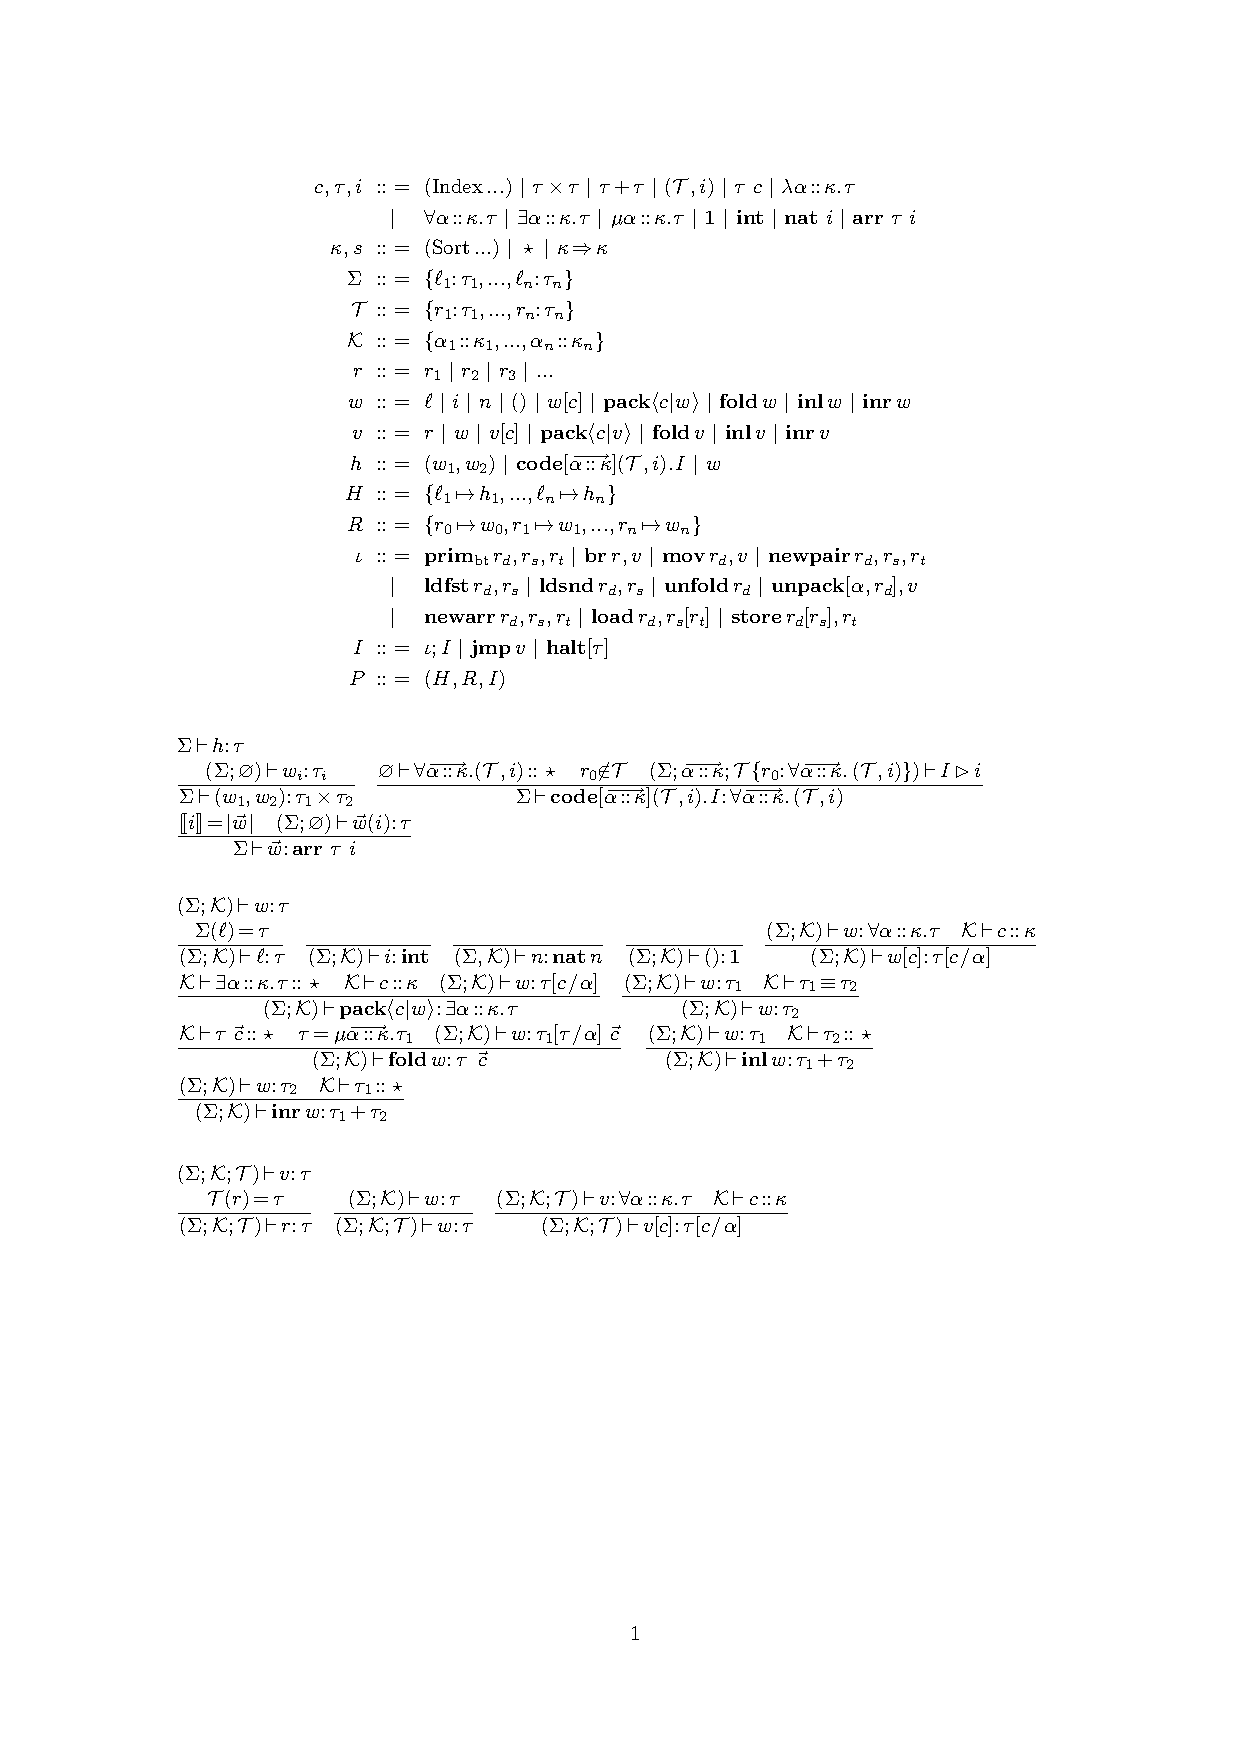
\includepdf[pages=-]{TiTAL}

\end{document}
